\documentclass[conference,a4paper,12pt]{IEEEtran}
\IEEEoverridecommandlockouts

\usepackage{graphicx}
\usepackage{url}

\begin{document}

\title{TCoin: A Cryptocurrency Based on Proof of Stake and Distributed Hash Table Networking}

\author{\IEEEauthorblockN{Naman Arora}
\IEEEauthorblockA{\textit{UFID: 3979-0439} \\
\textit{University of Florida}\\
naman.arora@ufl.edu}
\and
\IEEEauthorblockN{Gurupad Hegde}
\IEEEauthorblockA{\textit{UFID: 7835-6173} \\
\textit{University of Florida}\\
gmahabaleshwar@ufl.edu}
\and
\IEEEauthorblockN{Sourabh Gopal Parvatikar}
\IEEEauthorblockA{\textit{UFID: 7932-5142} \\
\textit{University of Florida}\\
sourabh.gopalpar@ufl.edu}
}

\maketitle

\begin{abstract}
In recent years, the boom of cryptocurrencies has led the way to a new field of study in Computer Science. A field that boasts a never before seen combination of Networking, Security and Economics. TCoin is a blockchain based cryptocurrency that tackles the \textit{Blockchain Trilemma} which has plagued this new field since its inception. TCoin is a novel way to approach the problems of decentralization, security and scalability and is inspired from a new type of consensus algorithm, Proof of Stake. It also focuses on changing the underlying networking model to a more scalable and fault tolerant Distributed Hash Table Network, Tapestry. TCoin has thus, been build from scratch to accommodate the amalgamation of these two very broad yet effective ideologies.
	
	The paper takes the reader through a brief introduction to the underlying concepts citing some relevant works and a bit of background introduction. Then the reader is presented with some interesting implementation details followed by some observations gathered from rigorous tests. These tests present a strong and compelling argument in favour of  TCoin. The paper ends by presenting some points that demand further research and development from the community.
\end{abstract}

\section{Introduction}
Blockchian technology, as put forth by Abadi \textit{et. al.} \cite{trilemma}, faces the problem of block chain trilemma. This means that either a blockchain can have security along with decentralized nature, but then would lack scalability, for eg. Bitcoin and Etherium. Or the blockchain can have scalability and decentralization, but then would have to be lax with security. This is, in part, the reason why most of the economics community could never accept blockchain based cryptocurrencies a \textit{de facto} standard. Moreover, severe threats to security, even with the likes of Bitcoin, have been discovered. Eclipse attacks \cite{eclipse}, possible deanonymization \cite{deanonymization_bitcoin}, partitioning attacks due to continual centralization \cite{partitioning} are all potential inhibitors to a global embrace of such a technology.
	
	TCoin was developed keeping in mind all the aforementioned problems and primarily focuses on providing a basis for further research in eliminating these threats. The two main features that TCoin boasts are, a completely revamped underlying network model and an upcoming consesus algorithm. The network is based on Distributed Hash Tables \cite{dht} dating back to the early 2000's. Consensus algorithm of Proof of Stake, on the other hand, is fairly new ideology and is currently under heavy scrutiny by the community. The mix of these techniques in a single use case is novel and thus requires a lot of community input.

\section{background}
\subsection{\textit{Tapestry, a DHT based P2P network}}
Distributed Hash Tables \cite{dht} provide a intuitive and fault tolerant path to peer to peer networking. Zaho \textit{et. al.} \cite{tapestry_dolr} \cite{tapestry_infra} picked up on that idea and pushed a new networking algorithm. This algorithm is based on hashing the peer's ID in the network and using that to route to it. For TCoin, we mainly focus on the DOLR API of tapestry explained as follows,
	\begin{itemize}
	\item{Peer References: }
	The node stores the peer hashes with addresses in the form of neighbour tables. These tables have levels, equal to the length of hash used for addressing. Each level maps to known peers with hashes having equal prefix upto a number greater than or equal to the level they currently are on.
	\item{Object References: }
	The objects, or in case of TCoin, transactions, are from the same pool as the ID hashes of nodes. The required object is routed to via IP CIDR type prefix matching algorithm by each successive node until the root of the object is not reached.
	\item{Object Root Node: }
	Each object present in the network is linked to a particular node in the network, currently existing or not. This helps in locating the object very easy with the help of object pointers, explained below.
	\item{Object Pointers: }
	To facilitate faster and more reliable object location, Tapestry stores references to the object's actual access location on each successive node in path to its route node. This makes locating the object very fast and efficient.
	\item{Publish and Un-publish Object: }
	Publishing an object basically means putting out object pointers with all the nodes in path to the object's root node. This make the object \textit{``available''} in the network. The Un-publishing is opposite to it. A node which has the object pointer might never receive un-publish broadcast and thus can have false information. Thus, Un-publish is best effort and does not guarantee anything.
	\item{Route to Node and Route to Object: }
	Route to an object is done by routing to that object's root node in the similar prefix matching fashion. As soon as a single pointer is found in any of the nodes along the path, the algorithm returns and the caller receives the connection information of the node.
	\end{itemize}
	
\subsection{\textit{Proof of Stake concensus algorithm}}
% \textit{\textit{Add Proof of stake algorithm here with 2-3 references}}
The idea of proof-of-work was first introduced in 1993 \cite{pvp} and was formally coined as proof-of-work in 1997. However, the idea went largely unused until Satoshi Nakamoto used this technique to create Bitcoin \cite{bitcoin_article}. Most cryptocurrencies like Bitcoin use enormous amount of electricity to secure their networks since mining coins requires a lot of computing power because of proof-of-work algorithm. In 2011 a Bitcointalk forum user called QuantumMechanic proposed a technique that he referred to as proof-of-stake \cite{bitcointalk}. PeerCoin \cite{peercoin} is the first crptocurrency to use proof-of-stake instead of proof-of-work.

The basic idea is that letting everyone compete against each other for mining in proof-of-work is wasteful. Therefore, proof-of-stake uses an election process in which one node is randomly chosen to validate the next block. Proof-of-stake has validators instead of miners and it does not let people mine blocks but instead, mint or forge blocks. Validators aren't chosen completely at random. To become a validator, a node has to deposit a certain amount of coins into the network as stake. The size of the stake determines the chances of a validator to be chosen to forge the next block. If a node is chosen to validate/forge the next block, it will check if all the transactions within it are valid. Upon successful validation, the validator node adds block to the blockchain. As a reward, the node receives the fees that are associated with each transaction. Validators lose a part of their stake if they approve fraudulent transactions. As long as validator's stake is higher than the reward, it can be trusted. This idea is a financial motivator and holds up as long as the stake is higher than the sum of all transaction fees. If a node stops being a validator, it's stake plus all the transaction fees that it received will not be released immediately, but after a certain period of time since the network needs time to check for fraudulent blocks in the blockchain, and punish the validator if it added those fraudulent blocks.

Proof-of-stake doesn't let everyone mine the blocks and therefore uses considerably less energy. Proof-of-stake is more decentralized than proof-of-work since there are no mining pools. Setting up a node for proof-of-stake based blockchain is a considerably less expensive compared to proof-of-work based blockchain.

\section{Architecture}
	\subsection{Transaction Algorithm}

	The transaction of currency between two individuals occurs when the source, \textit{A} has the wallet address of destination \textit{B}. \textit{A} can solicit the transaction by generating a TRA\_INIT request packet and publishing it according to the DOLR API \cite{tapestry_dolr} using the Route to Node function. When \textit{B} receives the request, it hashes the whole transaction contract and selects a validator using the validator selection algorithm (See subsection below). A validator \textit{C} is appointed for the validation process.

	The validator is oblivious to the amount involved in the contract and thus cannot form bias towards higher paying validation jobs. On being accepted as a legitimate stakeholder by \textit{B}, \textit{C} puts 50\% of the transaction amount as stake. The stake can be confiscated in the event of proven malpractice by \textit{C} and provided as an added incentive to the next validator that \textit{B} selects.

	On a successful validation, \textit{C} will cryptographically sign off the transaction and it will be published through usual DOLR \cite{tapestry_dolr} routine. In the event that the transactions don't checkout, transaction is cancelled and the stake of \textit{C} is released as is. This would certainly mean that the \textit{C's} resources are wasted, but is analogous to how in the Proof of Work, all miners mine for same block yet, only one is accepted. The incentive of successfully validating a transaction block is equivalent to 5\% of the total transaction amount. This incentive is charged from \textit{A} by \textit{B}.

	Since each node is associated to a unique hash, it can be mapped to its root node, again anonymous, using Tapestry's Route to Object algorithm. This root node would house just the latest transaction hash of the former node. In the event that a validator approaches this node for validation, it will provide the latest transaction hash. This would mean that each transaction hash is stored in two nodes, if at all available, first with the root node of the payee and second with the root node of the receiver. This leads to a very slight chance that the transaction can be counterfeit, as it is a testimony of two totally unconnected nodes. Note that, the real transaction contract is never stored anywhere but the node which received the money. The validator just gets that transaction contract's copy and reaches the root node to validate its hash and moves on to validate the same from the other root node. This is a vital process as a root node for one node can indeed become payee in a future transaction. Thus, it must be totally unaware of the origin of the transaction hashes it houses.

	\begin{figure}[h]
	  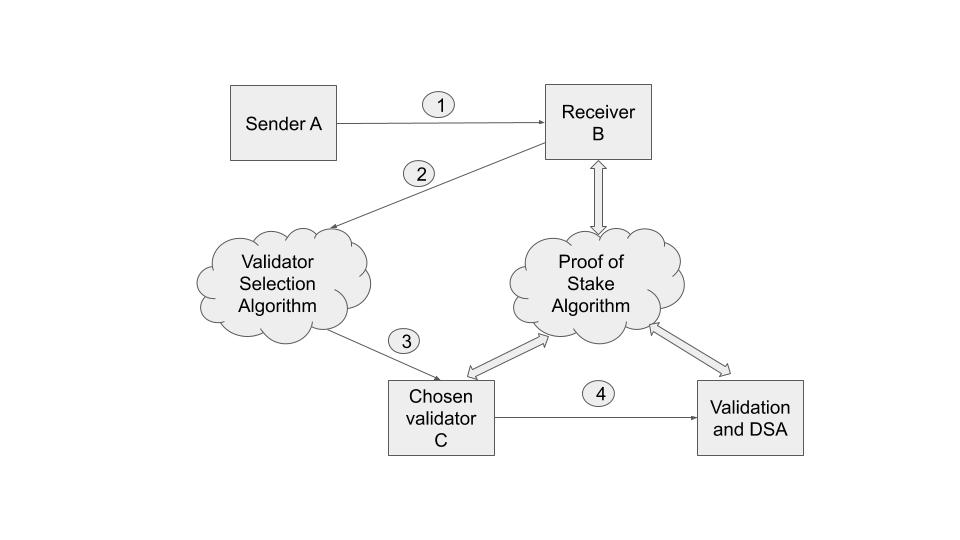
\includegraphics[width=\linewidth]{transaction_algo.jpg}
	  \caption{Transaction Algorithm Architecture}
	  \label{Transaction Architecture}
	\end{figure}

	\subsection{Validator Selection Algorithm}

	\begin{figure}[h]
	  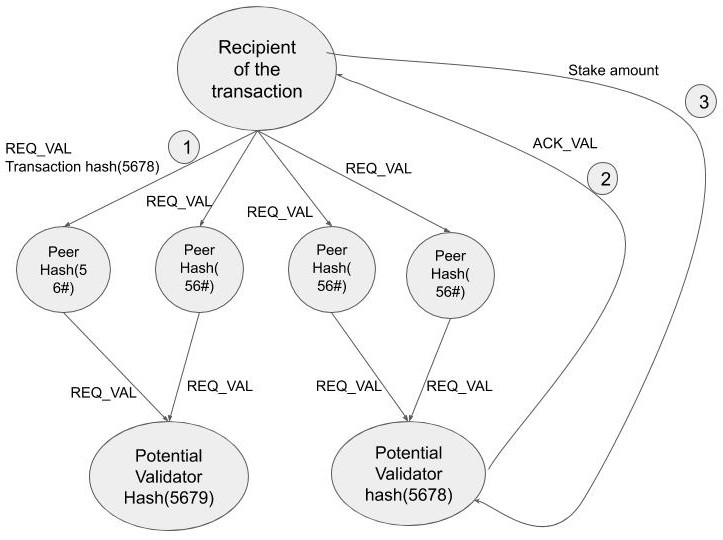
\includegraphics[width=\linewidth]{validation_algo.jpg}
	  \caption{Validation Algorithm Architecture}
	  \label{Validation Architecture}
	\end{figure}


	The validator is any node which can cryptographically sign off a transaction on the request of the receiver. This would lead to a 5\% incentive of the total transaction amount, but also requires 50\% of the amount to be kept as stake with the requester. The receiver has absolutely no say in selecting the validator. The selection algorithms again default to typical working of Tapestry \cite{tapestry_infra} as base.

	Suppose a transaction is initiated by \textit{A} in favour of \textit{B}. Now since \textit{B} has all the transaction details, it will hash them and publish a REQ\_VAL message towards the \textit{root} of that hash. All the nodes with wallet addresses along the route will respond to \textit{B's} request. These nodes are hereby referred to as \textit{potential validators}. The very first potential validator that shows up from \textit{B's} perspective, gets to start the deal.

	On selecting one of the potential validators, \textit{B} will then disclose the amount and the validator has to show at least 50\% of the total transaction's funds. The funds are in the form of previously signed transactions. If \textit{B} fails to verify the funds, the validator is rejected and the next one in the buffer is processed. On a successful validator selection, the stake is retained by \textit{B}.

	This validator selection algorithm can be initiated in one of the two cases:

	\begin{itemize}
    	\item A transaction within a group of individuals in favour of a single node.
	    \item At the time of network reboot, when a node needs to re validate its funds. 
	\end{itemize}


	\subsection{Transaction Renewal Process}
	
	This is one of key features of the currency. This allows the currency to be as anonymous as possible while maintaining a very shallow history so that scalability is never hindered. The whole network is required to reboot after a pre-determined amount of time. This would mean all the transactions before that point in time are deemed null and void. This would obviously require each node to re-validate its funds before the network reboot.

	This revalidation is done in the same way transactions between two individuals occur, \textit{i. e.} through Proof of Stake with the exception that this time, the node is generating a transaction from itself to itself. This reboot would mean that every node is audited by numerous other random nodes for the funds it claims to have. All the timestamps on the transactions \textit{need} to be greater than the latest reboot.

	The node looking to get its funds validated must choose a validator (See algorithm above). This validator node would submit the stake with the former node and on successful validation, get an incentive, just as always. In the event that a validator has stakes retained by another node and the network reaches the state of reboot, those stakes will be auto validated with the withholder as the person signing off. This would lead to no incentive for the withholder but a sort of free of cost validation for the former node.

\section{Implementation}

	TCoin is planned to be implemented in Elixir programming language \cite{elixir} which is the modern version of Erlang developed for the telecommunication industry. Elixir provides Actor model of concurrency in a very efficient and easy to understand coding pattern. The implementation involves developing three major modules,
	\begin{itemize}
	\item{Networking subsystem: }
	Comprised of Tapestry implementation in an easily usable API format.
	\item{Crypto Subsystem: }
	Comprised mostly of implementation of Proof of stake algorithm in the very unique fashion that TCoin hash.
	\item{The Main Driver Module: }
	This basically is the module that merges the last two into a full currency. Can be thought of a the wallet implementation.
	\end{itemize}
	
	\subsection{Networking Submodule}
	The Networking subsystem consists of three main modules, \textit{viz.}
	\begin{itemize}
	\item{The Node: }
	This acts like a handle to communicate for the Main Driver Module. Consider this as an interface to the whole Networking Subsystem. Each node is basically a GenServer module with its neighbour table as its persistent state. It has various overridden method definitions that a GenServer implements. The hashing of the \textit{process ID} provided by the Elixir/Erlang OTP is done using SHA256 algorithm. The hashed bits are encoded in hexadecimal notation and sliced off at eight characters, effectively locking the number of levels in each neighbour table to be equal to eight.
	\item{The Dispenser: }
	This module is an implementation technique. The Dispenser helps in setting up a new network of nodes and loses significance once an initial threshold of nodes is reached. This is a candidate for removal in future iterations of networking subsystem.
	\item{The DOLR API: }
	This is the module that will be exposed to the rest of the TCoin repository. This includes functions that can be used to interface with the whole networking machinery. The functions are:
		\begin{itemize}
			\item{Publish: }
			Inputs the \textit{transaction hash} to be published and the process ID of the node that is publishing it. It calculates the root node of the object and sends the object pointer along the way to the root node, simultaneously storing the object with itself.
			\item{Unpublish: }
			This also inputs the object to un-publish and the server process ID that is initiating the process of unpublication. But unlike publish, it instructs all the nodes down the line to delete their pointers.
			\item{Route to node: }
			Routing to a node requires the source and the destination process IDs to be provided. This passes along destination node's hash to its peers by traversing in prefix matching fashion.
			\item{Route to object: }
			This is just like Route to Node, but inputs the object hash the the destination instead.
			\item{Add: }
			This adds a node to the network when a new node joins in. It inputs the new node's process ID, its calculated hash and an entry point to the network.
		\end{itemize}
	\end{itemize}


\section{observations}
Now we describe our findings from the tests we ran on the completed Networking subsystem. The testing machine is equipped with Intel i7-8750H Hexcore, 12 Thread Mobile Laptop Processor with 16GB DDR4 memory .

	\subsection{Methodology}
	The experiment was run with two topologies, with 1000 and 2000 nodes each,
failing 5\%, 10\%, 15\% and 20\% of nodes totalling to 8 experimental runs. Each run
has been tested 5 times to provide consistency in output. All these functions are the
part of DOLR API.

	\subsection{Results}
	In our successive attempts to render the topology unusable, we have failed and thus
established its high degree of resilience.

The results are tabulated as following:

	\begin{figure}[h]
	  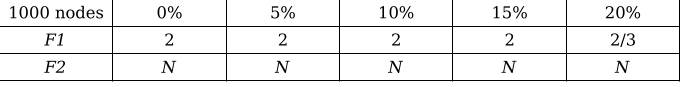
\includegraphics[width=\linewidth]{../observations/test_1000_nodes.png}
	  \caption{Table with results of 1000 nodes}
	  \label{Test 1}
	\end{figure}
	
	\begin{figure}[h]
	  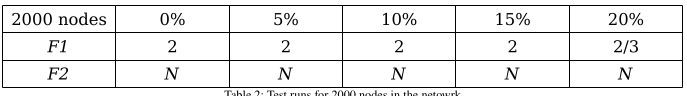
\includegraphics[width=\linewidth]{../observations/test_2000_nodes.png}
	  \caption{Table with results of 2000 nodes}
	  \label{Test 2}
	\end{figure}

F1 represents the route to object function call before un-publish and F2 represents the contrast.

Note that, the tables tabulate the Hops required to fetch the object. Also,
value of “N” shows that the object was never found. An uncertain value is
represented as ``\_/\_'' which shows the integral bounds of uncertainty.

\section{Further Steps}
The present work is just the beginning and TCoin can use a lot of further research attention. Some of the steps, that we acknowledge, that require such an attention are:
\begin{itemize}

\item{Completion of Crypto Subsystem.}
\item{Completion of Driver Subsystem.}
\item{Scaling of the blockchain over multiple physical nodes for measuring latency.}
\item{Latency and Transaction frequency analysis with TOR nodes attached.}
\item{Deliberate failure of nodes with most load to measure fault tolerance.}

\end{itemize}

\section{Conclusion}
TCoin is an effort to make the blockchain based cryptocurrencies mainstream. The firm belief that such a type of payment system, if made secure and scalable, can actually be a turning point in the history of economics. A lot of public expenditure on middlemen can be eliminated by making the system decentralized. Centralization leads to a single point of failure and at times is dangerous when economies of whole countries are at stake. Moreover, in the world with constant prying eyes and surveillance, this can actually be a panacea, much like Onion Routing is to networking. We thus, continue to strive for betterment of this technology and seek community input and criticism.

\newpage
\bibliography{references.bib} 
\bibliographystyle{ieeetr}

\end{document}